\documentclass[
  man,
  floatsintext,
  longtable,
  nolmodern,
  notxfonts,
  notimes,
  colorlinks=true,linkcolor=blue,citecolor=blue,urlcolor=blue]{apa7}

\usepackage{amsmath}
\usepackage{amssymb}




\RequirePackage{longtable}
\RequirePackage{threeparttablex}

\makeatletter
\renewcommand{\paragraph}{\@startsection{paragraph}{4}{\parindent}%
	{0\baselineskip \@plus 0.2ex \@minus 0.2ex}%
	{-.5em}%
	{\normalfont\normalsize\bfseries\typesectitle}}

\renewcommand{\subparagraph}[1]{\@startsection{subparagraph}{5}{0.5em}%
	{0\baselineskip \@plus 0.2ex \@minus 0.2ex}%
	{-\z@\relax}%
	{\normalfont\normalsize\bfseries\itshape\hspace{\parindent}{#1}\textit{\addperi}}{\relax}}
\makeatother




\usepackage{longtable, booktabs, multirow, multicol, colortbl, hhline, caption, array, float, xpatch}
\setcounter{topnumber}{2}
\setcounter{bottomnumber}{2}
\setcounter{totalnumber}{4}
\renewcommand{\topfraction}{0.85}
\renewcommand{\bottomfraction}{0.85}
\renewcommand{\textfraction}{0.15}
\renewcommand{\floatpagefraction}{0.7}

\usepackage{tcolorbox}
\tcbuselibrary{listings,theorems, breakable, skins}
\usepackage{fontawesome5}

\definecolor{quarto-callout-color}{HTML}{909090}
\definecolor{quarto-callout-note-color}{HTML}{0758E5}
\definecolor{quarto-callout-important-color}{HTML}{CC1914}
\definecolor{quarto-callout-warning-color}{HTML}{EB9113}
\definecolor{quarto-callout-tip-color}{HTML}{00A047}
\definecolor{quarto-callout-caution-color}{HTML}{FC5300}
\definecolor{quarto-callout-color-frame}{HTML}{ACACAC}
\definecolor{quarto-callout-note-color-frame}{HTML}{4582EC}
\definecolor{quarto-callout-important-color-frame}{HTML}{D9534F}
\definecolor{quarto-callout-warning-color-frame}{HTML}{F0AD4E}
\definecolor{quarto-callout-tip-color-frame}{HTML}{02B875}
\definecolor{quarto-callout-caution-color-frame}{HTML}{FD7E14}

%\newlength\Oldarrayrulewidth
%\newlength\Oldtabcolsep


\usepackage{hyperref}




\providecommand{\tightlist}{%
  \setlength{\itemsep}{0pt}\setlength{\parskip}{0pt}}
\usepackage{longtable,booktabs,array}
\usepackage{calc} % for calculating minipage widths
% Correct order of tables after \paragraph or \subparagraph
\usepackage{etoolbox}
\makeatletter
\patchcmd\longtable{\par}{\if@noskipsec\mbox{}\fi\par}{}{}
\makeatother
% Allow footnotes in longtable head/foot
\IfFileExists{footnotehyper.sty}{\usepackage{footnotehyper}}{\usepackage{footnote}}
\makesavenoteenv{longtable}

\usepackage{graphicx}
\makeatletter
\newsavebox\pandoc@box
\newcommand*\pandocbounded[1]{% scales image to fit in text height/width
  \sbox\pandoc@box{#1}%
  \Gscale@div\@tempa{\textheight}{\dimexpr\ht\pandoc@box+\dp\pandoc@box\relax}%
  \Gscale@div\@tempb{\linewidth}{\wd\pandoc@box}%
  \ifdim\@tempb\p@<\@tempa\p@\let\@tempa\@tempb\fi% select the smaller of both
  \ifdim\@tempa\p@<\p@\scalebox{\@tempa}{\usebox\pandoc@box}%
  \else\usebox{\pandoc@box}%
  \fi%
}
% Set default figure placement to htbp
\def\fps@figure{htbp}
\makeatother


% definitions for citeproc citations
\NewDocumentCommand\citeproctext{}{}
\NewDocumentCommand\citeproc{mm}{%
  \begingroup\def\citeproctext{#2}\cite{#1}\endgroup}
\makeatletter
 % allow citations to break across lines
 \let\@cite@ofmt\@firstofone
 % avoid brackets around text for \cite:
 \def\@biblabel#1{}
 \def\@cite#1#2{{#1\if@tempswa , #2\fi}}
\makeatother
\newlength{\cslhangindent}
\setlength{\cslhangindent}{1.5em}
\newlength{\csllabelwidth}
\setlength{\csllabelwidth}{3em}
\newenvironment{CSLReferences}[2] % #1 hanging-indent, #2 entry-spacing
 {\begin{list}{}{%
  \setlength{\itemindent}{0pt}
  \setlength{\leftmargin}{0pt}
  \setlength{\parsep}{0pt}
  % turn on hanging indent if param 1 is 1
  \ifodd #1
   \setlength{\leftmargin}{\cslhangindent}
   \setlength{\itemindent}{-1\cslhangindent}
  \fi
  % set entry spacing
  \setlength{\itemsep}{#2\baselineskip}}}
 {\end{list}}
\usepackage{calc}
\newcommand{\CSLBlock}[1]{\hfill\break\parbox[t]{\linewidth}{\strut\ignorespaces#1\strut}}
\newcommand{\CSLLeftMargin}[1]{\parbox[t]{\csllabelwidth}{\strut#1\strut}}
\newcommand{\CSLRightInline}[1]{\parbox[t]{\linewidth - \csllabelwidth}{\strut#1\strut}}
\newcommand{\CSLIndent}[1]{\hspace{\cslhangindent}#1}





\usepackage{newtx}

\defaultfontfeatures{Scale=MatchLowercase}
\defaultfontfeatures[\rmfamily]{Ligatures=TeX,Scale=1}





\title{Flattering Advice: Avoiding Disappointment in Advice-Giving}


\shorttitle{Flattering Advice}


\usepackage{etoolbox}









\authorsnames{Amanda Chen,David Hagmann}






\authorsaffiliations{
{Department of Management, The Hong Kong University of Science and
Technology},{}}




\leftheader{Chen and Hagmann}

\date{Invalid Date}


\abstract{Good advice improves decision quality but often requires
delivering unpleasant truths that may disappoint advisees. Across three
pre-registered and incentivized experiments involving real
adviser-advisee interactions (N = 3,900), we show that advisers
prioritize avoiding disappointment at the expense of accuracy and their
own earnings. In Study 1, advisers financially rewarded for accuracy
still tailor recommendations to aspirational goals expressed by
advisees, resulting in worse advice. When incentivized to be liked,
advisers provide even more flattering advice, and advisees reward this
by rating these advisers as more likable, despite the advice being less
honest and less accurate (Study 2). The desire to avoid disappointment
may lead to inequities if there are differences in expectations across
social groups. In Study 3, we examine a setting in which men expect to
perform better than women. We show that advisers take into account these
expectations, leading to systematically different advice for men and
women even when their gender is unknown to advisers. Advisers' efforts
to avoid disappointment may thus contribute to systematic gender
disparities in advice, with implications for downstream
decision-making.}

\keywords{Gender difference, Advice, Interpresonal relationship}

\authornote{\par{\addORCIDlink{Amanda
Chen}{0000-0002-4428-627X}}\par{\addORCIDlink{David
Hagmann}{0000-0002-2080-997X}} 

\par{       }
\par{Correspondence concerning this article should be addressed
to Amanda Chen, Email: zchengj@connect.ust.hk}
}

\makeatletter
\let\endoldlt\endlongtable
\def\endlongtable{
\hline
\endoldlt
}
\makeatother

\urlstyle{same}



\usepackage{float}
\usepackage{tabularray}
\usepackage[normalem]{ulem}
\usepackage{graphicx}
\UseTblrLibrary{booktabs}
\UseTblrLibrary{rotating}
\UseTblrLibrary{siunitx}
\NewTableCommand{\tinytableDefineColor}[3]{\definecolor{#1}{#2}{#3}}
\newcommand{\tinytableTabularrayUnderline}[1]{\underline{#1}}
\newcommand{\tinytableTabularrayStrikeout}[1]{\sout{#1}}
\makeatletter
\@ifpackageloaded{caption}{}{\usepackage{caption}}
\AtBeginDocument{%
\ifdefined\contentsname
  \renewcommand*\contentsname{Table of contents}
\else
  \newcommand\contentsname{Table of contents}
\fi
\ifdefined\listfigurename
  \renewcommand*\listfigurename{List of Figures}
\else
  \newcommand\listfigurename{List of Figures}
\fi
\ifdefined\listtablename
  \renewcommand*\listtablename{List of Tables}
\else
  \newcommand\listtablename{List of Tables}
\fi
\ifdefined\figurename
  \renewcommand*\figurename{Figure}
\else
  \newcommand\figurename{Figure}
\fi
\ifdefined\tablename
  \renewcommand*\tablename{Table}
\else
  \newcommand\tablename{Table}
\fi
}
\@ifpackageloaded{float}{}{\usepackage{float}}
\floatstyle{ruled}
\@ifundefined{c@chapter}{\newfloat{codelisting}{h}{lop}}{\newfloat{codelisting}{h}{lop}[chapter]}
\floatname{codelisting}{Listing}
\newcommand*\listoflistings{\listof{codelisting}{List of Listings}}
\makeatother
\makeatletter
\makeatother
\makeatletter
\@ifpackageloaded{caption}{}{\usepackage{caption}}
\@ifpackageloaded{subcaption}{}{\usepackage{subcaption}}
\makeatother

% From https://tex.stackexchange.com/a/645996/211326
%%% apa7 doesn't want to add appendix section titles in the toc
%%% let's make it do it
\makeatletter
\xpatchcmd{\appendix}
  {\par}
  {\addcontentsline{toc}{section}{\@currentlabelname}\par}
  {}{}
\makeatother

%% Disable longtable counter
%% https://tex.stackexchange.com/a/248395/211326

\usepackage{etoolbox}

\makeatletter
\patchcmd{\LT@caption}
  {\bgroup}
  {\bgroup\global\LTpatch@captiontrue}
  {}{}
\patchcmd{\longtable}
  {\par}
  {\par\global\LTpatch@captionfalse}
  {}{}
\apptocmd{\endlongtable}
  {\ifLTpatch@caption\else\addtocounter{table}{-1}\fi}
  {}{}
\newif\ifLTpatch@caption
\makeatother

\begin{document}

\maketitle


\setcounter{secnumdepth}{-\maxdimen} % remove section numbering

\setlength\LTleft{0pt}


\section{Introduction}\label{introduction}

Career trajectories for men and women often differ substantially, even
among those with similar qualifications. One source of such differences
may be the advice that people receive. Prior work has documented that
men receive more aspirational advice and women more risk-averse advice,
which may explain why women are less likely to apply for and ultimately
obtain more rewarding positions (Kanze et al., 2018). Research on gender
discrimination has focused on the role of unconscious bias (Banaji \&
Greenwald, 1995; Nosek et al., 2009), but interventions that try to
reduce this bias have been largely unsuccessful (Chang et al., 2019;
Paluck \& Green, 2009). Recent work has proposed cognitive, rather than
unconscious, biases that can lead to gender discrimination through the
formation of false beliefs (Hagmann et al., 2024). Here, we propose a
novel source of differences in advice by drawing on recent work on
belief-based utility, expectation-based reference points (Kőszegi \&
Rabin, 2006, 2009), and the hedonic consequences of information (Golman
et al., 2017).

Advice figures prominently in workplace and personal decision-making,
shaping choices about promotions, career paths, and everyday dilemmas
(Gino \& Moore, 2007; Harvey \& Fischer, 1997; Soll \& Larrick, 2009).
Its fundamental premise is to improve outcomes by enabling
decision-makers to learn from others' expertise. However, while honest
advice can lead to better decisions, it can also lead to disappointment
when it suggests a desired outcome is unlikely to materialize. Advisers
may be motivated to offer flattering recommendations that align with
advisees' hopes, sparing them the disappointment of a more sobering
forecast.

Advice with the potential for disappointment appears in diverse
organizational settings: supervisors deliver feedback on employee
performance, lawyers convey likely outcomes of litigation to their
clients, and academics offer thoughts on colleagues' manuscripts.
Ideally, honest information would help people identify their strengths
and weaknesses, make informed decisions about whether to pursue legal
cases, and strengthen papers prior to submission to academic journals,
thus improving long-term outcomes. In practice, however, interpersonal
considerations may prevent candor. When someone's expectations are (too)
high, an adviser might hesitate to deliver information that undermines
it---particularly if doing so risks negative interpersonal
repercussions.

People often go to great lengths to avoid unpleasant information,
deriving belief-based utility from maintaining favorable views of
themselves (Golman et al., 2017; Ho et al., 2021; Loewenstein \& Molnar,
2018). Moreover, they often prefer advisers who withhold bad news from
them (Shalvi et al., 2019) and punish those who communicate bad news
(John et al., 2019). Advisers, anticipating these preferences and
consequences face a dilemma: Should they provide the accurate but
potentially painful truth, or shade their recommendations to preserve
the advisee's mood and the adviser's own standing? Advisers who fear
they will be blamed or disliked for undermining someone's confidence may
reasonably avoid candid feedback, particularly if they don't incur a
cost when the advisee makes a mistake.

In our experiments, however, advisees have no opportunity to punish the
adviser, and advisers' financial incentives are linked to the decisions
the advisees make. We propose that advisers nonetheless have reason to
provide flattering advise because they recognize the psychological toll
of disappointing news. As a result, they may similarly incur a hedonic
cost for delivering unpleasant information that they anticipate may
distress the advisee. Thus, even in the anonymized context of an online
experiment, we hypothesize (and find) that advisers are relucant to
disappoint advisees and advice is thus biased upward, away from accuracy
and toward confirming advisees' priors. We show that this reduces the
quality of advice---but that advisees nonetheless view flattering
advisers more favorably.

We present the results of three preregistered experiments in which
participants are paired anonymously as advisers and advisees. Advisers
are incentivized to offer accurate advice, with bonus earnings depending
on the outcome of an advisee's decision. We study a setting in which
advisees can communicate their expectations to an adviser, and
experimentally manipulate whether advisers observe this expectation. Our
design simulates organizational contexts where mentors and managers
often have some sense of an employee's confidence or aspirations and
thus could adjust their feedback to avoid disappointing them.
Interpersonal considerations would likely be stronger in situations in
which the adviser and advisee have an existing relationship and when the
advice is delivered face-to-face. Moreover, advisers usually do not
suffer any direct costs when their flattering advice leads to a poor
outcome for the recipient, particularly when it is not clear what would
have happened under a counterfactual.\footnote{In some cases, however,
  repeated interaction might also increase incentives for honest
  feedback. Someone who is known to persistently give overoptimistic
  advice may be viewed as less trustworthy in the long run.}

In Study 1, we nudge advisees into a preference for competing against
either a group of top-performers or a group of low-performers, through
the use of a default option. Advisers who observe the actual performance
of advisees and therefore have the relevant information needed to make a
recommendation nonetheless take into account the initial preference when
recommending which group they should compete against. In Study 2, we ask
advisees to upload photos of themselves and advisers rank them on their
attractiveness. Advisers then recommend which rank the advisee should
bet on, receiving an incentive either for the advisee's accuracy or for
being evaluated favorably. Both groups of advisers recommend a rank that
is more attractive than what they themselves have evaluated the advisee,
and those incentivized for likability further inflate the ranking.
Advisees evaluate advisers more favorably when they recommend betting on
a more attractive rank, including viewing them as more trustworthy.

In Study 3, we examine a setting in which participants report their
expected performance on a mathematics quiz. Advisers observe the
test-taker's true score and, in one treatment, the score they guessed
they would receive. They then recommend whether the advisee should
compete against a group of high performers or low performers.
Importantly, this ``competition'' is based on the past performance
observed by the adviser and thus the advisee's expectation does not
provide instrumental information. However, we find that (1) men expect
to perform better than women, given identical performance, and (2)
advisers take these expectations into account. As a result, when
expectations (but not gender) are known to advisers, the advice given to
men and women differs, and men are more often advised to compete against
the group of high performers. Notably, this leads to worse advice for
men than for women.

\section{Open Science Statement}\label{open-science-statement}

We report all manipulations, measures, and data exclusion in our
experiments. The preregistration reports, screenshots of all
experimental materials, and the analysis code to replicate all
statistical analyses and figures are available on the Open Science
Framework
(\url{https://osf.io/8r3d4/?view_only=5ad7bafcd16b4d4ba08bb28b0e2bd02d}).

\section{Study 1}\label{study-1}

We first examine whether advisers take into account the expectations of
advisees when providing a recommendation. A group of participants
(``Advisees'') complete a quiz consisting of ten questions that draw on
ego-relevant domains. They then express a non-binding preference to
compete against a group of high performers or low performers on the same
task, based on their past performance. We nudge participants towards
picking either the low or the high performer group by selecting one of
the two by default. A second group of participants (``Advisers'')
observe Advisees' score on the quiz and, in one treatment, also which
group they had selected. We predicted that Advisees who were nudged
toward the high performer group would be more likely to receive advice
to compete against this high group when Advisers observed their
non-binding choice.

\subsection{Methods}\label{methods}

In a preliminary stage, we recruited 50 participants from Prolific and
gave them five minutes to complete a quiz consisting of ten items. The
quiz included word puzzles, identifying emotions from photos, and
selecting the best responses for hypothetical scenarios. These questions
were adapted from surveys that measure problem-solving, emotional
intelligence, and communication skills---which we pre-tested as being
important in modern society and hence where participants might have a
stake in doing well. Participants received a bonus of five cents for
each correctly answered question. We then ranked them based on their
score and label the 20 participants with the lowest (highest) scores as
the Low (High) Performer Group.

Next, we recruited 201 participants for the role of Advisees. They
completed the same 10-item quiz, also earning five cents for each
correct answer. We then asked them to express a non-binding preference
for whether they would like to compete against the High or Low Performer
Group. We informed them that they would be invited back at a later date
when they could make a binding decision and they could earn a bonus
based on whether their score on this quiz was equal to or higher than a
randomly selected member from their comparison group. If they picked the
High Performer Group and had an equal or higher score than a randomly
selected member of that group, they would earn a bonus of 50 cents. If
they picked the Low Performer Group and outperformed a randomly selected
member of that group, they could earn a bonus of 20 cents. If their
score was lower in this comparison, they would not earn an additional
bonus. We randomized which of the two groups (High or Low Performers)
was selected by default, and Advisees were free to select the other
group. They also made a guess as to their score, and the survey
concluded with basic demographic questions.

We then recruited 1,000 participants for the role of Advisers, and the
focal part of our experiment. They were informed of the ability quiz
that the Advisees had completed, how the Low Performer Group and High
Performer Groups were constructed, as well as the choice and incentives
for the Advisees. We then asked Advisers to give advice to ten
participants on which group they should compete against. Advisers were
randomly assigned to one of two treatments. In the ``Performance''
treatment, they observed only the score of the other participant. In the
``Performance + Expectation'' treatment, they additionally observed the
advisee's non-binding choice of which group to compete against. However,
since the outcome was based solely on the past quiz score and advisers,
but not advisees, know the score, this initial choice was not
informative for the purpose of recommending competing against one group
or the other. Advisers could earn the same bonus as one of the
participants they had given advice to and who returned to make a
decision. The survey concluded with basic demographic questions.

Finally, we invited Advisees back for the follow-up survey. Following
our preregistration, we kept the survey open for 7 days. In total, 176
Advisees returned. The short survey reminded them of the task they
completed in the previous survey, informed them that other participants
from Prolific had observed their real score and given them advice on
which group to compete against, and finally reminded them of how many
questions they guessed they had answered correctly. They were not
informed of their true score or the score of the groups they could
compete against. Participants then observed the advice from a randomly
selected adviser and made their decision.

\subsection{Results}\label{results}

We begin by examining the performance of the Stage 1 participants.
Because our default treatment takes place after participants completed
the ability quiz, we do not expect a difference in performance across
the Low and High Default treatments. Indeed, the two groups score no
different from one another (5.10 and 5.18 for the Low Default and High
Default treatments, respectively, \(t(199) = 0.31\), \(p = .756\)). As
expected, the default manipulation changes their initial choices. In the
``Low Default'' treatment, only 22\% of participants prefer to compete
against the High Performer Group, compared to 65\% of participants in
the ``High Default'' treatment (\(\chi^2\)(1, n = 201) = 36.62, p
\textless{} .001).

\linespread{1}

\begin{table}

{\caption{{Advice to compete against the High Performer Group in Study
1. Displaying the non-binding choice of those for whom the Low Performer
Group was selected by default makes it less likely that they are advised
to compete against the High Performer Group (Column 1). Column 2
restricts the analysis to advisers who observe advisees' initial
non-binding choice and controls for advisees' score on the quiz.
Standard errors are clustered at the adviser
level.}{\label{tbl-study1regs}}}\vspace{0pt}
}

\centering
\begin{talltblr}[         %% tabularray outer open
entry=none,label=none,
note{}={+ p \num{< 0.1}, * p \num{< 0.05}, ** p \num{< 0.01}, *** p \num{< 0.001}},
]                     %% tabularray outer close
{                     %% tabularray inner open
colspec={Q[]Q[]Q[]},
column{3}={}{halign=c,},
column{1}={}{halign=l,},
cell{2}{2}={}{halign=c,},
cell{3}{2}={}{halign=c,},
cell{4}{2}={}{halign=c,},
cell{5}{2}={}{halign=c,},
cell{6}{2}={}{halign=c,},
cell{7}{2}={}{halign=c,},
cell{8}{2}={}{halign=c,},
cell{9}{2}={}{halign=c,},
cell{10}{2}={}{halign=c,},
cell{11}{2}={}{halign=c,},
cell{12}{2}={}{halign=c,},
cell{13}{2}={}{halign=c,},
cell{1}{2}={c=2,}{halign=c, halign=c,},
hline{13}={1,2,3}{solid, black, 0.05em},
}                     %% tabularray inner close
\toprule
& Advice to Compete Against High Performers &  \\ \cmidrule[lr]{2-3}
& All Advice & Expectations Shown \\ \midrule %% TinyTableHeader
High Default               & \num{0.011}    & \num{0.025}*    \\
& (\num{0.013})  & (\num{0.011})   \\
Expectation Shown          & \num{-0.041}*  &                  \\
& (\num{0.016})  &                  \\
Expectation x High Default & \num{0.037}+   &                  \\
& (\num{0.019})  &                  \\
Score                      &                 & \num{0.168}***  \\
&                 & (\num{0.004})   \\
Constant                   & \num{0.389}*** & \num{-0.503}*** \\
& (\num{0.012})  & (\num{0.020})   \\
N                          & \num{10000}    & \num{5000}      \\
\bottomrule
\end{talltblr}

\end{table}

We now examine whether advisers take the advisees' expectations into
account. Advisers observe the true performance of the advisee, such that
expectations about performance add no additional information. However,
because participants who score higher are also more likely to pick the
High Performer Group, we use our Default treatment as an instrument that
reflect higher expectations. We show linear probability models for the
decision of the Advisers, which is equal to 1 if they recommend
competing against the High Performer Group and 0 if they recommend the
Low Performer Group. In Column 1 of Table~\ref{tbl-study1regs}, we show
our main specificiation with the experimental assignment for Advisees
(High Performer Default vs.~Low Performer Default) and Advisers
(Expectation Shown vs.~Expectation Hidden), as well as their
interaction. Because each adviser made ten recommendations, we cluster
standard errors at the adviser level. We find that displaying
expectations of those in the Low Performer Default reduces
recommendations to compete against the Top group by 4 percentage points,
or about 10\% relative to when expectations are hidden. This decrease is
marginally smaller for advisees with a default choice to compete against
the High Performer Group (nudged to have high expectations, though not
necessarily holding them), and whose advice did not differ based on
whether their expectations were shown or hidden. We reported a linear
probability model on advising to compete against the High Performer
group for advisers in the ``Expectations'' treatment, controlling for
the true performance of the advisee in Column 2 of
Table~\ref{tbl-study1regs}. We observe a significant main effect of the
default treatment, where a high default increased the likelihood of
receiving flattering advice. It is worth noting that, since only 65 \%
of advisees in the high default group actually stuck with their default
choice, this represents a conservative test of the effect of high
expectations on the likelihood of receiving flattering advice.

\begin{figure}

\caption{\label{fig-study1Advice}Advice given in Study 1. Advisees who
were nudged to express high expectations were more likely to receive
advice to compete against the High Performer Group.}

\centering{

\pandocbounded{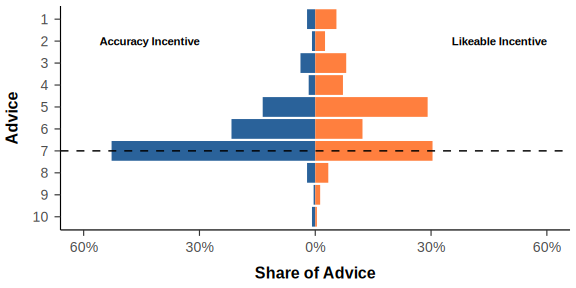
\includegraphics[keepaspectratio]{manuscript_files/figure-pdf/fig-study1Advice-1.pdf}}

}

\end{figure}%

\subsection{Discussion}\label{discussion}

When an adviser knows an outcome that an advisee can only estimate,
learning this estimate should not change the advice that is given.
However, in line with our argument that advisers take into account the
belief utility of the advisee and prefer to avoid disappointing them, we
find that providing information about expectations makes a difference.
Specifically, advisees who expressed a preference for stronger
competitors were more likely to receive flattering advice, encouraging
them to pursue that option. This occurs even though advisers are
incentivized to give good advice.

\section{Study 2}\label{study-2}

We next examine if advisers believe that flattering advice will improve
how they are perceived, and if so, whether this perception is true. We
do this by manipulating the incentives for advisers, who receive a bonus
either based on how they are evaluated by an advisee, or a bonus for the
advisee's accuracy.

The study takes place in three stages. First, a group of advisees upload
photos of themselves (``selfies'') and are grouped with nine other
participants of the same sex We then recruit participants of the
opposing sex to rank them from most to least attractive and to provide
advice. Specifically, they advise the participant they ranked as the 7th
most attractive (i.e., 4th least attractive) on what rank they should
bet they were ranked by a larger group of raters. Advisers were randomly
assigned to two treatments, receiving a bonus payment either if the
advisee guessed their rank accurately or if the advisee evaluated the
adviser as likeable as measured by a scale response. We hypothesize that
advisers incentivized to be liked will recommend betting on a lower
rank, i.e.~that the advisee is more attractive.

\subsection{Methods}\label{methods-1}

We recruit 300 participants from Prolific and, after asking demographic
questions, invite them to upload photos of themselves (selfies) to be
rated by other participants on attractiveness. We obtain selfies from
100 men and 107 women adhering to our instructions (e.g., did not
include other people). In line with our preregistration, we select the
first 100 photos from women to arrive at a gender-balanced sample
(\(M_{\text{Age}}\) = 39.37 years). Participants are informed that their
selfies will be randomly grouped with those of nine other participants
of their sex and ranked in terms of attractiveness by a group of new
Prolific participants of the opposite sex. They then make an
unincentivized guess of their rank.

Next, we recruit 472 participants from Prolific for the role of advisers
(\(M_{\text{Age}}\) = 41.0275424 years; 49.79\% Female). We first
collect demographic information, then match them to a group of the
opposite sex. They rank selfies from ten participants from most to least
attractive using a drop-down menu next to each picture. Because of a
limitation with the survey software, we could not validate that each
rank is given only once, and we remove 115 participants who failed to
follow instructions and did not provide a complete ranking.\footnote{Moreover,
  we could not collect data from any participant who did not select any
  participant as the 7th most attractive participant, as that image
  would be shown on subsequent pages.}

After submitting their ratings, participants see the photo of the
participant they ranked as the 7th most attractive (i.e., the 4th least
attractive). We remind them of the rank they have just given to that
person and inform them that this participant will be invited back and
can earn a \$1 bonus if they correctly guess their rank. The rank is
determined by the aggregate ratings of all participants who have ranked
this group. Because the participant does not observe the other nine
people in the group, they would depend on the adviser's recommendation
along with their own assessment. We randomly assign advisers to one of
two incentivization schemes. In the ``Accuracy'' treatment, they receive
a bonus identical to the advisee: \$1 if they guess their rank
correctly. In the ``Likeability'' treatment, we inform them that the
advisee will rate them on a 5-point Likert scale on how likeable they
thought they are. Each point on the scale would translate to a bonus of
20 cents. Advisers then select a rank (from 1 to 10) that they recommend
the advisee to bet on.

Finally, we invite participants from Stage 1 who were ranked as the 7th
most attractive participant by at least one adviser (so that they
received advice) back for the follow-up survey. Following our
preregistration, we keep the survey open for 7 days. In total, 146
participants (77 men, 69 women) complete the follow-up survey. We remind
them of the selfie they uploaded in Stage 1 and that a group of 10
selfies, including theirs, had been rated by other participants from
Prolific. They then see the advice from a randomly selected adviser and
make their own guess with a \$1 incentive for accuracy. Finally, they
rate the adviser's likability, warmth, friendliness, good-naturedness,
trustworthiness, and sincerity on 5-point Likert scales (adapted from
Fiske et al., 2007).

\subsection{Results}\label{results-1}

\begin{figure}

\caption{\label{fig-study2advice}Participants in Study 2 give advice to
the person they rank 7th most attractive out of 10. When incentivized
for accuracy, the majority recommends betting on that rank. However,
when incentivized for likeability, participants inflate their advice to
flatter the recipient as more attractive.}

\centering{

\pandocbounded{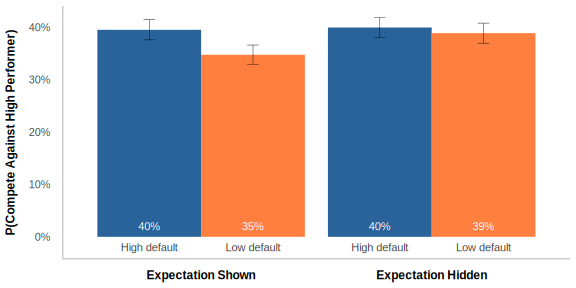
\includegraphics[keepaspectratio]{manuscript_files/figure-pdf/fig-study2advice-1.pdf}}

}

\end{figure}%

We begin by examining the prior beliefs of advisees who uploaded their
selfies. On average, men guess they rank 5.76 in their group of 10 and
women guess that they rank 6.37 (\(t(205) = 2.15\), \(p = .033\)).
Notably, people's self-perceptions correlate strongly with the aggregate
ratings of the advisers (0.43, \(t(193) = 6.70\), \(p < .001\)).
However, there is substantial heterogeneity in perceptions of
attractiveness. Of the 200 participants, 149 are ranked as 7th most
attractive by at least one adviser. On average, men in this subset
estimate they rank 5.94th and women estimate they rank 6.59th
(\(t(143) = 1.94\), \(p = .054\)).

Next, we turn our attention to the advisers (see
Figure~\ref{fig-study2advice}). In the Accuracy condition, those
uploading selfies are on average advised to bet on rank 6.19. Notably,
this is significantly more attractive than the 7th rank those advisers
had themselves guessed just on the prior screen (\(t(234) = -8.82\),
\(p < .001\)). This suggests that even when incentivized for accuracy,
participants offer flattering advice.\footnote{This shading could be due
  to concerns of avoiding disappointment. However, it could also be that
  advisers are uncertain about the rankings they have given and make a
  recommendation that combines their own belief with a uniform prior.
  Therefore, our analyses focus on the difference between the two
  conditions.} Importantly, and as predicted, we find that advisers in
the Likeable treatment recommend betting on a lower rank, communicating
that they think the participant in the selfie is more attractive (5.38,
\(t(470) = 5.44\), \(p < .001\)). This suggests that advisers infer
flattering someone with pleasant advice would make the adviser appear
more likeable. The distribution shown in Figure~\ref{fig-study2advice}
shows that participants do not simply tell participants that they are
the most attractive person in the group. They may infer that flattering
advise needs to be somewhat realistic to be believable. We return to
this in the general discussion.

\begin{table}

{\caption{{When individuals receive advice that implies a high level of
attractiveness (lower rank), they tend to perceive the advice giver as
more likable (Column 1), warm (Column 2). Column 3 shows that advisors
are rated as more trustworthy when they advice lower ranks, but this
relationship is only directional.}{\label{tbl-study2regs}}}\vspace{0pt}
}

\centering
\begin{talltblr}[         %% tabularray outer open
entry=none,label=none,
note{}={+ p \num{< 0.1}, * p \num{< 0.05}, ** p \num{< 0.01}, *** p \num{< 0.001}},
]                     %% tabularray outer close
{                     %% tabularray inner open
colspec={Q[]Q[]Q[]Q[]},
column{2,3,4}={}{halign=c,},
column{1}={}{halign=l,},
hline{6}={1,2,3,4}{solid, black, 0.05em},
}                     %% tabularray inner close
\toprule
& (1) & (2) & (3) \\ \midrule %% TinyTableHeader
Advised Rank & \num{-0.109}*  & \num{-0.133}** & \num{-0.054}   \\
& (\num{0.046})  & (\num{0.044})  & (\num{0.042})  \\
Constant     & \num{3.777}*** & \num{3.903}*** & \num{3.397}*** \\
& (\num{0.279})  & (\num{0.266})  & (\num{0.257})  \\
N            & \num{146}      & \num{146}      & \num{146}      \\
\bottomrule
\end{talltblr}

\end{table}

Finally, we examine whether flattering advice indeed leads to more
positive evaluations of advisers, or whether flattering advice is
dismissed as insencere. Following our preregistration, we average the
ratings on likeability, warmth, friendliness, and good-naturedness to
create a scale of likeability (\(\alpha\) = 0.9243334); and we create a
scale of trustworthiness by averaging the ratings of trustworthiness and
sincerity (\(\alpha\) = 0.8740347).

\begin{figure}

\caption{\label{fig-study2rating}Participants tend to rate advisors who
suggest betting on a higher rank (implying greater attractiveness) as
more likable and warm.}

\centering{

\pandocbounded{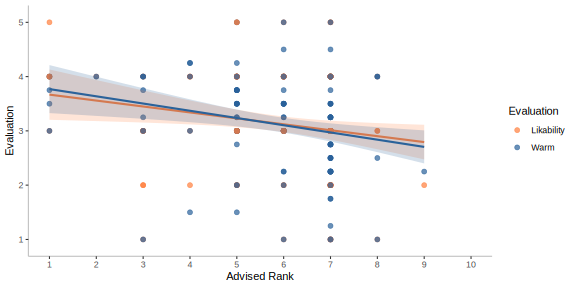
\includegraphics[keepaspectratio]{manuscript_files/figure-pdf/fig-study2rating-1.pdf}}

}

\end{figure}%

\begin{figure}

\caption{\label{fig-study2ratingByGroup}After participants receive
advice that suggests betting on a rank that was lower than, equal to, or
higher than their own guess, they evaluate advisors based on their
likability and warmth. Participants rate advisors who give flattering
advice and deliver a high evaluation of their attractiveness as more
likable and warm than those whose advice implied a lower evaluation of
their attractiveness.}

\centering{

\pandocbounded{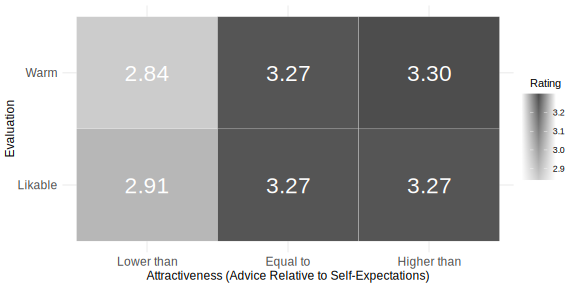
\includegraphics[keepaspectratio]{manuscript_files/figure-pdf/fig-study2ratingByGroup-1.pdf}}

}

\end{figure}%

As seen in Figure~\ref{fig-study2rating}, we advisers who suggested that
the advisee was more attractive (lower rank) were indeed rated as more
likeable and warm (b = -0.109, p \textless{} .05; b = -0.133, p
\textless{} .001, respectively; See Columns 1 and 2 of
Table~\ref{tbl-study2regs}). When using their own initial guess as a
reference point, advisers who suggest a worse rank are perceived as less
likable and warm (see Figure~\ref{fig-study2ratingByGroup}).
Interestingly, these benefits are not at the cost of sincerity; advisers
who recommend a more favorable rank are viewed as no less trustworthy
(Column 3 of Table~\ref{tbl-study2regs}).

We are not powered to do a comparison across the two experimental groups
and did not preregister such a difference. Indeed, we find no difference
in likeability and warmth across the two treatments (\(t(144) = 1.09\),
\(p = .275\), and \(t(144) = 0.58\), \(p = .562\), respectively). We
also assess the quality of advice by measuring the discrepancy between
the advised rank and the correct rank. We find no difference in accuracy
across the advice treatments (\(t(144) = -0.29\), \(p = .776\)).

\subsection{Discussion}\label{discussion-1}

In another context where advice communicates ego-relevant information
(here, people's attractiveness), we find that the advice people give is
contingent on their incentives. Specifically, when they get rewarded for
being more likeable, they recommend that the advisee bet on a more
favorable rank than when they are incentivized for accuracy.
Importantly, advisees do not discount flattering advice and instead
evaluate people who advise them to bet on a more attractive rank as
warmer and more likeable. These gains to interpersonal perceptions do
not come at the cost of trustworthiness, even when the advice is
inflated.

\section{Study 3}\label{study-3}

In Study 3, we examine how advisers who want to avoid disappointment may
inadvertently contribute to gender differences in advice. We ask
participants to estimate their score on a mathematics test, and
anticipate that men will guess higher than women. Moreover, we expect
that advisers take into account the expected score when recommending
whether someone should compete against a group of High or Low
performers. As a result, we hypothesize that, when expectations are
known to advisers, men will be advised to compete against High
Performers more than women, even when advisers do not know gender and
expectations are uninformative.

\subsection{Methods}\label{methods-2}

We begin by first recruiting a sample of 50 participants from Prolific
to complete a 10-question multiple choice mathematics quiz. The
questions are taken from a paper-version of the ASVAB standardized exam,
such that answers are not available online. Participants have five
minutes to answer the quiz and are paid 10 cents for each correctly
answered question. Like in Study 1, we define the top 20 scores as
``High Performers'' and the bottom 20 scorers as the ``Low Performers.''
On average, participants answered 4.42 questions correctly, High
Performers scored between 5 and 10, and Low Performers scored between 0
and 3. In order to anchor the expectations of participants in our main
experiment, we simulated 1,000 pairings of groups of five participants,
with the 5th percentile of groups scoring an average of 2.6 and the 95
th percentile scoring an average of 6.4. We report these averages to
participants in the Low Expectations and High Expectations treatment,
respectively.

We then recruit 1,002 participants for the role of advisees in Stage 1
of our main experiment. To arrive at a gender-balanced sample, we drop
the last two male participants to complete the survey, ending up with a
sample of 500 men and 500 women (\(M_{\text{Age}}\) = 42.16).
Participants complete the same 10-item mathematics quiz as the earlier
participants and are informed that their performance would affect their
bonus earnings in a follow-up stage to be conducted a few days later.
After completing the quiz, we inform them of the average score of a
group of five participants from the preliminary survey. We randomly
assign them to learn about the 5th percentile of groups, which scored
2.6. (``Low Expectations'' treatment) or the 95th percentile of groups,
which scored 6.4 (``High Expectations'' treatment). Participants then
make an unincentivized guess about how many questions they think they
answered correctly. The survey concludes with basic demographic
questions.

We then recruit 1,000 participants for Stage 2, placing them in the role
of advisers. We begin by informing them of the mathematics quiz that
participants in the preliminary study and Stage 1 have completed, and
inform them of the average score of all participants in the preliminary
study. Advisers have to recommend whether an advisee should compete
against the Low Performers or the High Performers (we use these terms in
the survey). We anticipate that being told to compete against High
Performers is more flattering and hence being told to compete against
the Low Performers would be disappointing if one had expected to do
well. Advisees would earn a bonus if their score is equal to or higher
than that of a randomly selected member from their chosen group. They
earn 50 cents if they outperform a High Performer and 30 cents if they
outperform a Low Performer.

Advisers are randomly assigned to one of two treatments. In the
``Baseline'' treatment, they only observe the score of the advisee on
the mathematics quiz. In the ``Expectation'' treatment, they observe the
score as well as the advisee's guess for how many questions they
answered correctly. Since the outcome is determined only by the past
score on the quiz, the advisee's guess is not informative for the
recommendation, which can be based on the revealed score. Moreover, in
neither treatment did they receive any demographic information about the
advisees. Participants give recommendations to 10 advisees, which
unbeknownst to them are five men and five women matched to have
identical performance on the test.\footnote{We made this decision to
  account for the possibility of gender differences in performance.}
They are informed that if their advice is shown to a participant who
returns for the follow-up survey, they will receive the identical bonus
as that participant. The survey then concludes with basic demographic
questions.

Finally, we invite participants from Stage 1 back for the follow-up
survey. Following our preregistration, we keep the survey open for seven
days. In total, 951 participants (481 men, 470 women) return. The brief
survey reminds them of the task they completed in Stage 1, informs them
that other participants from Prolific have observed their real score and
given them advice on which group to compete against, and finally are
reminded of how many questions they guessed they had answered correctly.
Importantly, they are not informed of their true score or the score of
the groups they could compete against. Participants then observe the
advice from a randomly selected adviser and make their decision.

\subsection{Results}\label{results-2}

We begin by examining the performance of the Stage 1 participants.
Because our treatment takes place after participants complete the
mathematics quiz, we would not expect a difference in performance across
the Low and High Expectations treatments. Indeed, the two groups score
no different from one another (4.79 and 4.55 for the Low Expectations
and High Expectations treatments, respectively, \(t(998) = -1.64\),
\(p = .102\)). As intended, the expectations treatment does affect how
well they thought they performed. Participants in the ``Low
Expectations'' treatment guess a score of 4.79 vs. 4.42 in the High
Expectations treatment (\(t(998) = 3.78\), \(p < .001\)), showing that
the manipulation is successful, albeit small. Contrary to our
expectations, we find a gender difference in performance: men score 5.02
on average, while women score 4.33 (\(t(998) = -4.73\), \(p < .001\)).
Consistent with this difference, men think they answered more questions
correctly than do women (4.75 vs 3.56, \(t(998) = -8.60\),
\(p < .001\)). This difference, however, does not affect the
interpretation of our findings, which will rely on an interaction of
gender with an experimental treatment for Stage 2 participants.

We define a measure of ``overconfidence'' as (Performance - Estimate).
We observe that women underestimate their performance by 0.76 points,
while men do so by only 0.27 points (\(\Delta M = -0.49\), 95\% CI
\([-0.73, -0.25]\), \(t(997.87) = -4.03\), \(p < .001\)). Although
neither gender is overconfident, men on average are more confident in
their performance than are women, as we had expected.

\begin{table}

{\caption{{Column 1 displays the advice given to compete against a High
Performance group based on whether the advisees were primed with low or
high expectations and the expectation level shown to the advisor. Column
2 displays the advice given to compete against a High Performance group
based on the gender of the targets and the expectation level shown to
the advisor. Column 3 displays the expected bonus of the advice received
based on the gender of the targets and the expectation level shown to
the advisor. All standard errors clustered at the level of the
advisor.}{\label{tbl-study3regs}}}\vspace{0pt}
}

\centering
\begin{talltblr}[         %% tabularray outer open
entry=none,label=none,
note{}={+ p \num{< 0.1}, * p \num{< 0.05}, ** p \num{< 0.01}, *** p \num{< 0.001}},
]                     %% tabularray outer close
{                     %% tabularray inner open
colspec={Q[]Q[]Q[]Q[]},
column{2,3,4}={}{halign=c,},
column{1}={}{halign=l,},
hline{14}={1,2,3,4}{solid, black, 0.05em},
}                     %% tabularray inner close
\toprule
& (1) & (2) & (3) \\ \midrule %% TinyTableHeader
High Expectation   & \num{0.012}     &                 &                 \\
& (\num{0.011})   &                 &                 \\
Performance        & \num{0.128}***  &                 &                 \\
& (\num{0.003})   &                 &                 \\
Expectation Shown  &                  & \num{-0.034}*  & \num{0.000}    \\
&                  & (\num{0.013})  & (\num{0.003})  \\
Advisee Male       &                  & \num{0.002}    & \num{0.000}    \\
&                  & (\num{0.005})  & (\num{0.001})  \\
Expectation x Male &                  & \num{0.032}*** & \num{-0.005}** \\
&                  & (\num{0.009})  & (\num{0.002})  \\
Constant           & \num{-0.263}*** & \num{0.339}*** & \num{0.258}*** \\
& (\num{0.015})   & (\num{0.010})  & (\num{0.002})  \\
N                  & \num{5000}      & \num{10000}    & \num{10000}    \\
\bottomrule
\end{talltblr}

\end{table}

\begin{figure}

\caption{\label{fig-study3genderdiff}Advisers observed real performance
and the participants' estimated performance, but not their gender. As a
result of their higher expectations, men (blue) were advised to compete
against the high performance group more often than women (red). The grey
line shows advice absent expectations, which did not differ by gender.}

\centering{

\pandocbounded{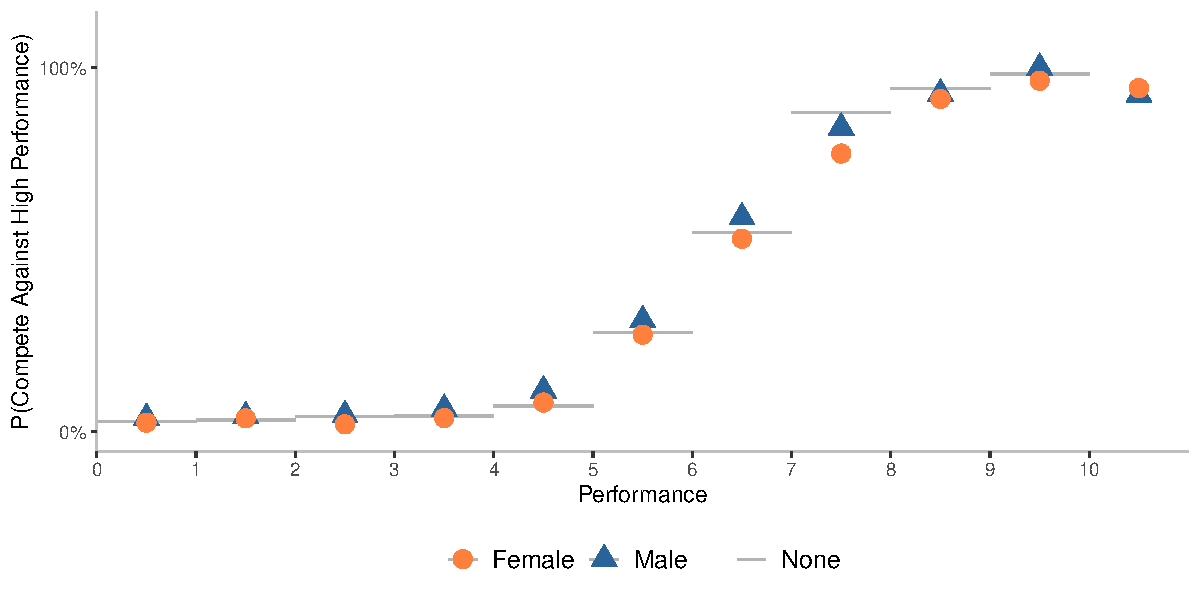
\includegraphics[keepaspectratio]{manuscript_files/figure-pdf/fig-study3genderdiff-1.pdf}}

}

\end{figure}%

Next, we examine whether advisers take the advisee's expectations into
account. Column 1 of Table~\ref{tbl-study3regs} reports a linear
probability model on advising to compete against the High Performer
group for advisers in the ``Expectations'' treatment, controlling for
the true performance of the advisee. Because each adviser makes ten
recommendations, we cluster standard errors at the adviser level.
However, contrary to our expectations, we do not see a significant
effect of the expectations treatment. This may be because the induced
difference in expectations was too small.

However, recall that men are more confident in their performance than
are women. Our theory thus predicts that showing expectations should
lead to more flattering advice (i.e., a recommendation to compete
against the High Performer group) for men than for women. We report a
linear probability model with advice to compete against the high group
as the outcome measure, and the advisee's gender, whether expectations
were shown to the adviser, and the interaction of the two in Column 2 of
Table~\ref{tbl-study3regs}. As predicted, we find a significant
interaction effect: men are more likely to be advised to compete against
the High Performers when expectations are shown than when they are
hidden (\(p < 0.001\)). We show this result graphically in
Figure~\ref{fig-study3genderdiff}. As the figure makes clear, this
effect is driven by advice given to those who scored in the middle of
the possible range. Thus, when it is clear that someone should compete
against Low or High performers, advisers are not deferring to
expectations.

To examine the quality of advice, we computed the expected bonus
earnings for someone who follows the recommendations. For example, if an
adviser suggests competing against the High Performer group, we match
the advisee against all 20 members of that group and determined how
often their score matches or exceeds that of the member. We then
multiply this number by the respective bonus earnings (50 cents and 30
cents for the High and Low Performer group, respectively). To see if
including expectations leads to worse advise for men, we report a linear
probability model with the experimental treatment of the adviser, the
gender of the advisee, and their interaction in Column 3 of
Table~\ref{tbl-study3regs}. Displaying expectations leads men to be
advised to compete against the High Performer group more often, and this
advice turns out to be costly: men receive worse advise than do women
when expectations are displayed, but not in their absence.\footnote{This
  analysis was not preregistered, and we note here that the reduction in
  expected earnings is small. However, it is interesting that
  expectations have a negative effect for men who underestimate their
  performance on average. One possibility is that advisers suggest the
  High Performer group more often than is optimal. This is consistent
  with our finding from Study 2, in which participants offered
  flattering advice even when incentivized only for accuracy.}

\begin{table}

{\caption{{Column 1 displays the actual bonus based on the performance
and whether the participant is primed with high expectations. Column 2
displays the actual bonus based on the performance and gender of the
participant. Columns 3 and 4 display the chance of adopting the advice
based on the gender of the participants, whether the advisee sees
expectations, and whether the advice is to compete against high
performers. The former considers only the main effect, while the latter
also includes the interactive
effect.}{\label{tbl-study3time3}}}\vspace{0pt}
}

\centering
\begin{talltblr}[         %% tabularray outer open
entry=none,label=none,
note{}={+ p \num{< 0.1}, * p \num{< 0.05}, ** p \num{< 0.01}, *** p \num{< 0.001}},
]                     %% tabularray outer close
{                     %% tabularray inner open
colspec={Q[]Q[]Q[]Q[]Q[]},
column{2,3,4,5}={}{halign=c,},
column{1}={}{halign=l,},
hline{20}={1,2,3,4,5}{solid, black, 0.05em},
}                     %% tabularray inner close
\toprule
& (1) & (2) & (3) & (4) \\ \midrule %% TinyTableHeader
Performance                          & \num{0.038}*** & \num{0.039}*** &                  &                  \\
& (\num{0.003})  & (\num{0.003})  &                  &                  \\
High Expectation                     & \num{-0.020}   &                 &                  &                  \\
& (\num{0.013})  &                 &                  &                  \\
Advisee Male                         &                 & \num{-0.002}   & \num{-0.045}+   & \num{-0.144}*** \\
&                 & (\num{0.013})  & (\num{0.026})   & (\num{0.041})   \\
Expectation x Male                   &                 &                 &                  & \num{0.113}*    \\
&                 &                 &                  & (\num{0.053})   \\
Expectation Shown                    &                 &                 & \num{-0.002}    & \num{-0.057}    \\
&                 &                 & (\num{0.026})   & (\num{0.040})   \\
Advice: High Performer               &                 &                 & \num{-0.138}*** & \num{-0.207}*** \\
&                 &                 & (\num{0.028})   & (\num{0.051})   \\
Advice: High Performer x Male        &                 &                 &                  & \num{0.131}*    \\
&                 &                 &                  & (\num{0.056})   \\
Expectation x Advice: High Performer &                 &                 &                  & \num{-0.009}    \\
&                 &                 &                  & (\num{0.056})   \\
Constant                             & \num{0.087}*** & \num{0.076}*** & \num{0.857}***  & \num{0.906}***  \\
& (\num{0.016})  & (\num{0.015})  & (\num{0.024})   & (\num{0.030})   \\
N                                    & \num{483}      & \num{483}      & \num{951}       & \num{951}       \\
\bottomrule
\end{talltblr}

\end{table}

To determine whether flattering advice is truly costly, however, we need
to examine the outcome of the advisees. In particular, they could ignore
flattering advice, recognizing it as such and thus failing to adhere to
it. In line with our prediction, participants who are primed with high
expectations earn less when their expectations are shown to the
advisers, although this result is only directional (see Column 1 of
Table~\ref{tbl-study3time3}). Similarly, as shown in Column 2 of
Table~\ref{tbl-study3time3}, we also find that male participants earn
less when their expectations are shown. These findings suggest that
flattering advice is not without consequences. Furthermore, our research
indicates that because men are more likely to follow such advice (see
Column 4 of Table~\ref{tbl-study3time3}), they compete more as a result
of flattering advice.

\subsection{Discussion}\label{discussion-2}

Our findings suggest that attempts to avoid disappointment can be a
novel source of gender differences in advice. Women underestimate their
mathematics test scores more than men. When these expectations are shown
to advisors, they are more likely to tell men to compete against high
performers than women. Notably, this turns out to be poor advice: men
whose advisors are aware of their expectations receive worse advice. Our
findings suggest that men with the same scores as their female
counterparts end up earning less, although this result is only
directional. This discrepancy may be due to men receiving more favorable
advice, being more likely to follow it, and ultimately facing worse
outcomes.

\section{General Discussion}\label{general-discussion}

Advice has the potential to shape people's career and personal outcomes.
Honest feedback, however, may be painful to learn if it falls short of
one's expectations. As prior work notes, this may motivate people to
avoid information and avoid seeking help (Bénabou et al., 2022; Golman
et al., 2017; Jaroszewicz et al., 2021). We present evidence from three
experiments that advisers are also cognizant of this cost. As a result,
they present flattering advice that avoids disappointing the recipient,
and correctly anticipate that this boosts how advisees perceive them.
However, this flattering advice comes at a cost to advisees, who would
do worse if they followed it blindly.

Moreover, a desire to avoid disappointment also means that advisers have
to take into account the expectations of the advisee. We document that
men are more optimistic about their performance than women are. As a
result, they receive more flattering advice and are more likely to be
told to aim higher. Notably, in the context of our experiment, this
turns out to be bad advice ex post.

Our findings have implications for organizational practice, where
mentoring and advice-giving may take into account an employees'
expectation. We document this as a novel source of gender bias.
Organizations could reduce this bias by calibrating employees'
expectations to reduce overconfidence.

Participants in our experiment were paired anonymously. Even so, we
document this desire to avoid disappointment. We anticipate that advice
would be more flattering in face-to-face communication and without
anonymity. Moreover, existing relationships might make it even more
difficult for advisers to be honest.

In our experiments, participants only received advice once and did not
evaluate the adviser after observing the outcome of their decision. For
example, advice that leads to bad outcomes may undermine the
interpersonal benefits of flattery. Alternatively, people may still like
the flattering advice and not fault the adviser for the bad outcome.
Moreover, our setting involved only a single piece of advice on one
task. Future research could examine whether people return to those who
gave them flattering advice, or if they prefer someone who gave them the
honest (but unpleasant) truth.

Advice has long been studied from the perspective of the receiver.
Similarly, research on belief utility has examined how recipients
respond to the valence of the information they receive. Here, we show
that advisers, too, take into account the psychological impact of the
information they convey. They may have even greater motivations to avoid
conveying bad news, because they incur the interpersonal costs of
delivering unfavorable information without reaping the benefits from
helping someone make a better choice.

\section{References}\label{references}

\phantomsection\label{refs}
\begin{CSLReferences}{1}{0}
\bibitem[\citeproctext]{ref-Greenwald1995}
Banaji, M. R., \& Greenwald, A. G. (1995). Implicit gender stereotyping
in judgments of fame. \emph{Journal of Personality and Social
Psychology}, \emph{68}(2), 181.

\bibitem[\citeproctext]{ref-Benabou2022}
Bénabou, R., Jaroszewicz, A., \& Loewenstein, G. (2022). \emph{It
{Hurts} to {Ask}}. National Bureau of Economic Research.

\bibitem[\citeproctext]{ref-Chang2019}
Chang, E. H., Milkman, K. L., Gromet, D. M., Rebele, R. W., Massey, C.,
Duckworth, A. L., \& Grant, A. M. (2019). The mixed effects of online
diversity training. \emph{Proceedings of the National Academy of
Sciences}, \emph{116}(16), 7778--7783.

\bibitem[\citeproctext]{ref-Fiske2007}
Fiske, S. T., Cuddy, A. J., \& Glick, P. (2007). Universal dimensions of
social cognition: Warmth and competence. \emph{Trends in Cognitive
Sciences}, \emph{11}(2), 77--83.

\bibitem[\citeproctext]{ref-Gino2007}
Gino, F., \& Moore, D. A. (2007). Effects of task difficulty on use of
advice. \emph{Journal of Behavioral Decision Making}, \emph{20}(1),
21--35.

\bibitem[\citeproctext]{ref-Golman2017}
Golman, R., Hagmann, D., \& Loewenstein, G. (2017). Information
avoidance. \emph{Journal of Economic Literature}, \emph{55}(1), 96--135.
\url{https://doi.org/10.1257/jel.20151245}

\bibitem[\citeproctext]{ref-Hagmann2024}
Hagmann, D., Sajons, G. B., \& Tinsley, C. H. (2024). \emph{Base rate
neglect as a source of inaccurate statistical discrimination}.

\bibitem[\citeproctext]{ref-Harvey1997}
Harvey, N., \& Fischer, I. (1997). Taking advice: {Accepting} help,
improving judgment, and sharing responsibility. \emph{Organizational
Behavior and Human Decision Processes}, \emph{70}(2), 117--133.

\bibitem[\citeproctext]{ref-Ho2018}
Ho, E. H., Hagmann, D., \& Loewenstein, G. (2021). Measuring information
preferences. \emph{Management Science}, \emph{67}(1), 126--145.

\bibitem[\citeproctext]{ref-Jaroszewicz2022}
Jaroszewicz, A., Loewenstein, G., \& Bénabou, R. (2021). \emph{The pain
of asking and being asked for informal help}.

\bibitem[\citeproctext]{ref-John2019}
John, L. K., Jeong, M., Gino, F., \& Huang, L. (2019). The
self-presentational consequences of upholding one's stance in spite of
the evidence. \emph{Organizational Behavior and Human Decision
Processes}, \emph{154}, 1--14.

\bibitem[\citeproctext]{ref-Kanze2018}
Kanze, D., Huang, L., Conley, M. A., \& Higgins, E. T. (2018). We ask
men to win and women not to lose: {Closing} the gender gap in startup
funding. \emph{Academy of Management Journal}, \emph{61}(2), 586--614.

\bibitem[\citeproctext]{ref-Koszegi2006}
Kőszegi, B., \& Rabin, M. (2006). A model of reference-dependent
preferences. \emph{The Quarterly Journal of Economics}, \emph{121}(4),
1133--1165.

\bibitem[\citeproctext]{ref-Koszegi2009}
Kőszegi, B., \& Rabin, M. (2009). Reference-dependent consumption plans.
\emph{American Economic Review}, \emph{99}(3), 909--936.

\bibitem[\citeproctext]{ref-Loewenstein2018}
Loewenstein, G., \& Molnar, A. (2018). The renaissance of belief-based
utility in economics. \emph{Nature Human Behaviour}, \emph{2}(3),
166--167.

\bibitem[\citeproctext]{ref-Greenwald2009}
Nosek, B. A., Smyth, F. L., Sriram, N., Lindner, N. M., Devos, T.,
Ayala, A., Bar-Anan, Y., Bergh, R., Cai, H., Gonsalkorale, K., et al.
(2009). National differences in gender--science stereotypes predict
national sex differences in science and math achievement.
\emph{Proceedings of the National Academy of Sciences}, \emph{106}(26),
10593--10597.

\bibitem[\citeproctext]{ref-Paluck2009}
Paluck, E. L., \& Green, D. P. (2009). Prejudice reduction: What works?
A review and assessment of research and practice. \emph{Annual Review of
Psychology}, \emph{60}, 339--367.

\bibitem[\citeproctext]{ref-Shalvi2019}
Shalvi, S., Soraperra, I., Weele, J. J. van der, \& Villeval, M. C.
(2019). \emph{Shooting the messenger? Supply and demand in markets for
willful ignorance}.

\bibitem[\citeproctext]{ref-Soll2009}
Soll, J. B., \& Larrick, R. P. (2009). Strategies for revising judgment:
How (and how well) people use others' opinions. \emph{Journal of
Experimental Psychology: Learning, Memory, and Cognition}, \emph{35}(3),
780.

\end{CSLReferences}






\end{document}
